\chapter{Evaluation} \label{evaluation}

\section{Life-Like CA}

When evaluating the effectiveness of evolutionary techniques at learning life-like CA rules, it is important to contextualise quantitative properties like convergence rate, fitness, and diversity. We begin by performing an exploratory statistical analysis to gather data on the life-like CA rule space. In conjunction with the analyses of Wolfram\cite{wolfram1986theory} and Eppstein\cite{eppstein2010growth}, this will shed light into the characteristics that make a rule easier or harder to predict.

\section{Exploratory Analysis}
There are $2^{18} = 262144$ possible outer-totalistic cellular automata rules which makes a systematic analysis feasible through random simulation. This is a useful way to map properties of the rulespace so that we can evaluate  100 initial conditions are sampled from a distribution uniform across densities 0 to 1. Each rule is simulated on each initial condition for 100 time steps and the state at each step is recorded in a hashmap. If a state previously visited at time step $t$ is produced again at step $t+\delta$, the rule is said to have converged at $t+\delta$ time steps with period $\delta$. We examine each rule to find the percentage of initial conditions that converge within 100 steps and the mean oscillation period of those that converge.\\

First we consider the two extremeties. 23.2\% of rules converge for all initial conditions and 49.8\% of rules converge for only 2 out 100 initial conditions. Note this is the minimum convergence number in our setting since all rules will converge for the trivial initial conditions with density 0 and density 1. The proof of this is detailed in \ref{quiescent-nullity}. This leaves 27.0\% or 70708 of the original rules remaining. While the original dataset had a median of 3\% convergence, the reduced set of rules present a more even spread with a median of 13\%.

\begin{definition}[Quiescence]
A CA is quiescent if all cells are in the same state. A CA with each cell $c_i$ in state $\sigma_i(t) = 0$ is denoted $\vec{0}$ and the opposite quiescent CA with $\sigma_i(t) = 1$ is denoted $\vec{1}$. 
\end{definition}

\begin{lemma}
A quiescent life-like CA is at a fixed point or oscillates with period 2.   
\end{lemma}

\begin{proof} \label{quiescent-nullity}
Consider an arbitrary cell $c_i$ in $\vec{0}$. $\sigma_i(0) = 0 \text{\ and\ } n_i(t) = 0$\\
\begin{multicols}{2}
\noindent If $0 \notin B$:\\
\null \quad $\sigma_i(1) = 0 \text{\ and\ } n_i(1) = 0 $\\
\null \quad $\implies$ convergence to $\vec{0}$ with period 1.\\
\columnbreak\linebreak
\noindent If $0 \in B$:\\
\null \quad $\sigma_i(1) = 1 \text{\ and\ } n_i(1) = 8 $\\
\null \quad If $8 \in S$:\\
\null \qquad $\sigma_i(2) = 1 \text{\ and\ } n_i(1) = 8 $\\
\null \qquad $\implies$ convergence to $\vec{1}$ with period 1.\\
\null \quad If $8 \notin S$:\\
\null \qquad $\sigma_i(2) = 0 \text{\ and\ } n_i(1) = 0 $\\
\null \qquad $\implies$ oscillation between $\vec{0}$ and $\vec{1}$.
\end{multicols}
\noindent The case for a CA at quiescent state $\vec{1}$ is exactly symmetrical.
\end{proof}

\begin{figure}[!h]
\centering
            \subfloat{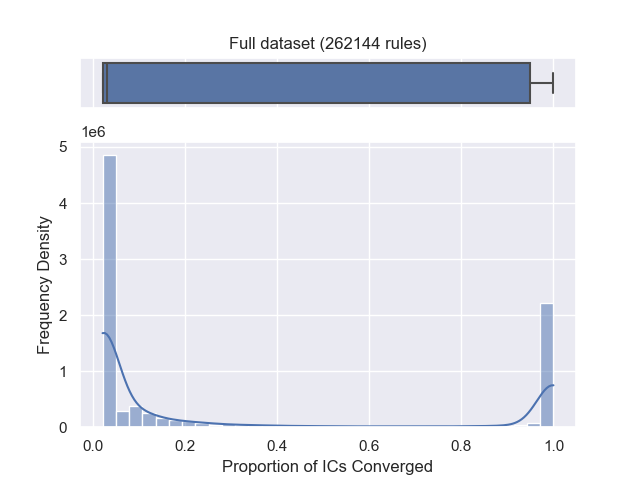
\includegraphics[width=.5\textwidth]{images/full-taxonomy.png}}\hfill
            \subfloat{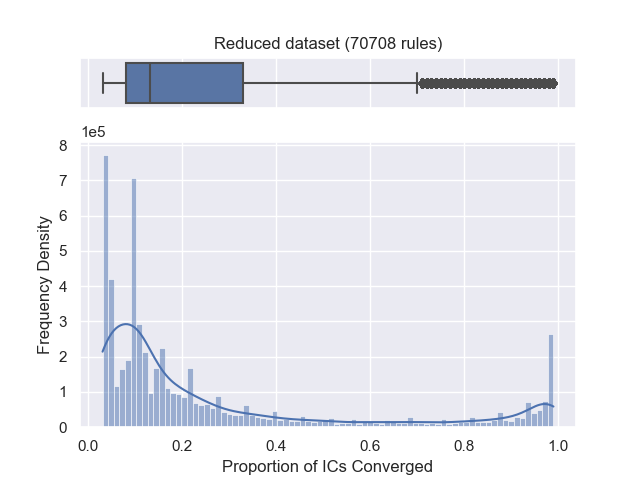
\includegraphics[width=.5\textwidth]{images/reduced-taxonomy.png}}\hfill
            \caption{Distributions of convergence of full and reduced set of life-like CAs}
\label{fig:taxonomy-dist}
\end{figure}

\section{Hyperparameter Tuning}

We begin by performing some crude hyperparameter testing on the genetic algorithm. Considering a random uniform stepsize, $\delta_k \sim \mathit{Uniform}(D_{max}, D_{min})$ we set $D_{min} = 1$ since we would like to give the algorithm a chance of learning on very small steps. To determine $D_{max}$, the algorithm is run on 100 goal rules and each the loss of each rule is calculated by simulating on 100 random initial conditions. By running the algorithm on populations of size 10 and 100 with $D_{max} \in \{1, 10, 100\}$ for 30 epochs, we find the highest proportion of experiments converging to the precise goal rule within 30 epochs when the population is of size 100 and $D_{max}$ is 10. With this configuration, 32\% of goals are precisely learnt. It is clear that population size makes a considerable difference on performance so for all future tests, we maintain a population size of 100.

\begin{figure}[!h]
\centering
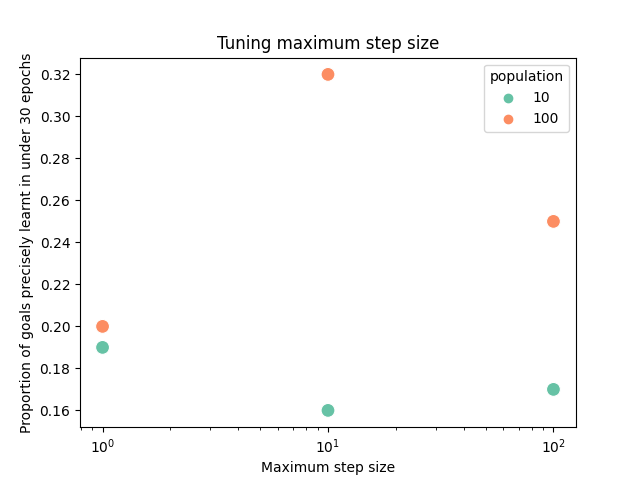
\includegraphics[width=0.7\textwidth]{images/tune-max-step.png}
\caption{Percentage of runs that converge within 30 epochs}
\label{fig:tune-max-step}
\end{figure}

In order to reduce training time when testing different hyperparameters, we reduce the size of the training set of initial conditions from 100 to 20. Although this somewhat compromises on the strength of the overall algorithm, it allows us to quickly compare multiple different configurations. One such choice is between loss functions. We consider the performance of the single resolution loss against the multiple resolution loss on a population of 100 over 30 epochs with 20 random initial conditions tested per individual.\\    

